\chapter{Architecture Design Guidelines}

\section{Leading requirements}

The following list of leading requirements is meant to guide the creation and maintenance
of design guidelines and design decisions. The most important requirements are first
and foremost leading arguments in any comparison of alternatives. 

\begin{description}

	\item[Portability leads] We need the design tool to run equally well on all defined platforms
	and possibly platforms not (yet) defined. For that reason portability is a leading requirement.
	
	\item[Ease of use seconds] We need the design tool to assist in the design of \Noc and
	the development of verification tools with respect to \Noc designs. For that reason the design
	tool should facilitate these activities as much as possible. 
	
	\item[Maintainability third] The ease of maintenance was one of the primary requirements and
	as such should guide future design decisions. 
	
	\item[Performance follows] Under normal circumstances performance arguments should not lead.
	However, unacceptable performance will override all other considerations, because
	unacceptable performance disrupts use of the tool. 
	
	\item[Remark] What is acceptable performance is subjective. 
	
\end{description}

\paragraph{Example} When given a choice between alternatives with equal portability and 
ease of use consequences, the maintenance arguments should lead at the cost of performance 
provided the performance seems acceptable.

\paragraph{Agreement} On 6th December 2014 Bernard agreed to this priority ordering. 

\section{High level design guidelines}

\begin{description}

	\item[C++ constructs lead] We strive to use C++ of the latest standard, currently C++ 2011.
	This implies the use of the C++ library including containers.
	
	\item[qt] We use the GUI library \qt for all GUI code and as much other code as is necessary.
	
	\item[OpenGL] For drawing 2D we use qtquick1 with graphicsview or qtquick2 which works with opengl.
	It looks like we will be using qtquick1 with graphicsview due to some missing features (scrol, zoom, 
	pan) in qtquick2.

	\item[Other libraries] We use \qt as our goto library for portability. For mechanisms that would
	otherwise require platform dependent code we use \qt. Messaging, process control and
	interprocess communication is all directed through \qt. Only if \qt does not suffice do we
	use other libraries like \boost.
	
	
\end{description}

\section{Observer pattern}

The observer pattern is described in the \w{GoF} \citep{Gamma:1995:DPE:186897}. 
Figure \ref{fig:observer-applied} shows an implementation of 
the pattern that applies the principle as 
described in the book.

\begin{center}
	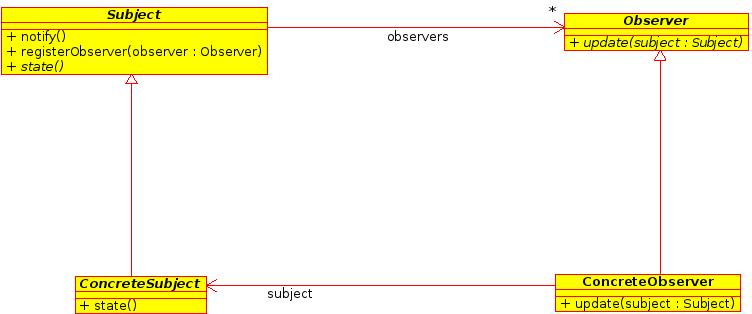
\includegraphics[width=.7\linewidth]{ObserverClassDiagram.jpeg}
	\captionof{figure}{Observer pattern as described in \w{GoF}}
	\label{fig:observer-pattern}
\end{center}

\begin{center}
	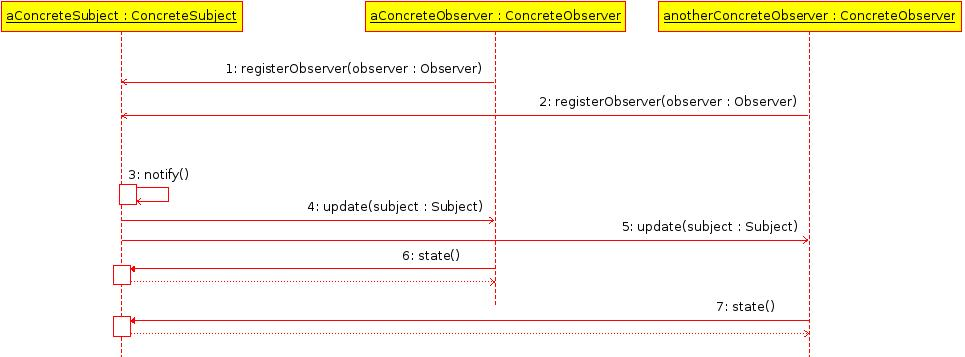
\includegraphics[width=.7\linewidth]{ObserverSequenceDiagram.jpeg}
	\captionof{figure}{Observer pattern applied}
	\label{fig:observer-applied}
\end{center}

The toolkit \qt provides signals and slots for communication 
between objects in a \qt based system. It is a fundamental mechanism to bind 
together classes that do not know of each other's existance.

We use this mechanism in place of the observer pattern because it is
simple and needs no additional programming other than the \code{connect()} 
statement and the slot method.

The mechanism works as follows:

\begin{enumerate}
	\item A class emits a signal. Any slot connected to the signal
	will be executed as a result. This is a one-to-many relationship.
	Each signal can connect to multiple slots.	
	
	\item Many signals can connect to a slot. When any of these signals 
	emit this will cause the slot to execute. This is a many-to-one relationship.
	Each slot can have connections from multiple signals.
	
	\item Any signal $s_1$ can connect to any other signal $s_2$. The result of
	emitting the $s_1$ will be a subsequent emission of $s_2$.
	
	\item When an object is removed, existing connections it contains are deleted 
	by the \qt system.
	
\end{enumerate}

The slots are normal methods with return values (that the signals ignore) and 
parameters. The connection processes the parameters only if the signal and the 
slot have the same parameters with the same types. If they do not, the system 
ignores the parameters. Any method can call the slots (this is where the return
value comes in). 

Besides the graphical system that uses signals and slots extensively, we can use
signals and slots in any class that specifies the \qobj macro. This enables
inter process communication.

